\section{Performance Optimierung auf DBMS-Ebene}

In diesem Kapitel soll es darum gehen, wie das DBMS Queries möglichst performant ausführt und wie wir diese Ausführung analysieren und beeinflussen können.

\subsection{Puffermanagement}

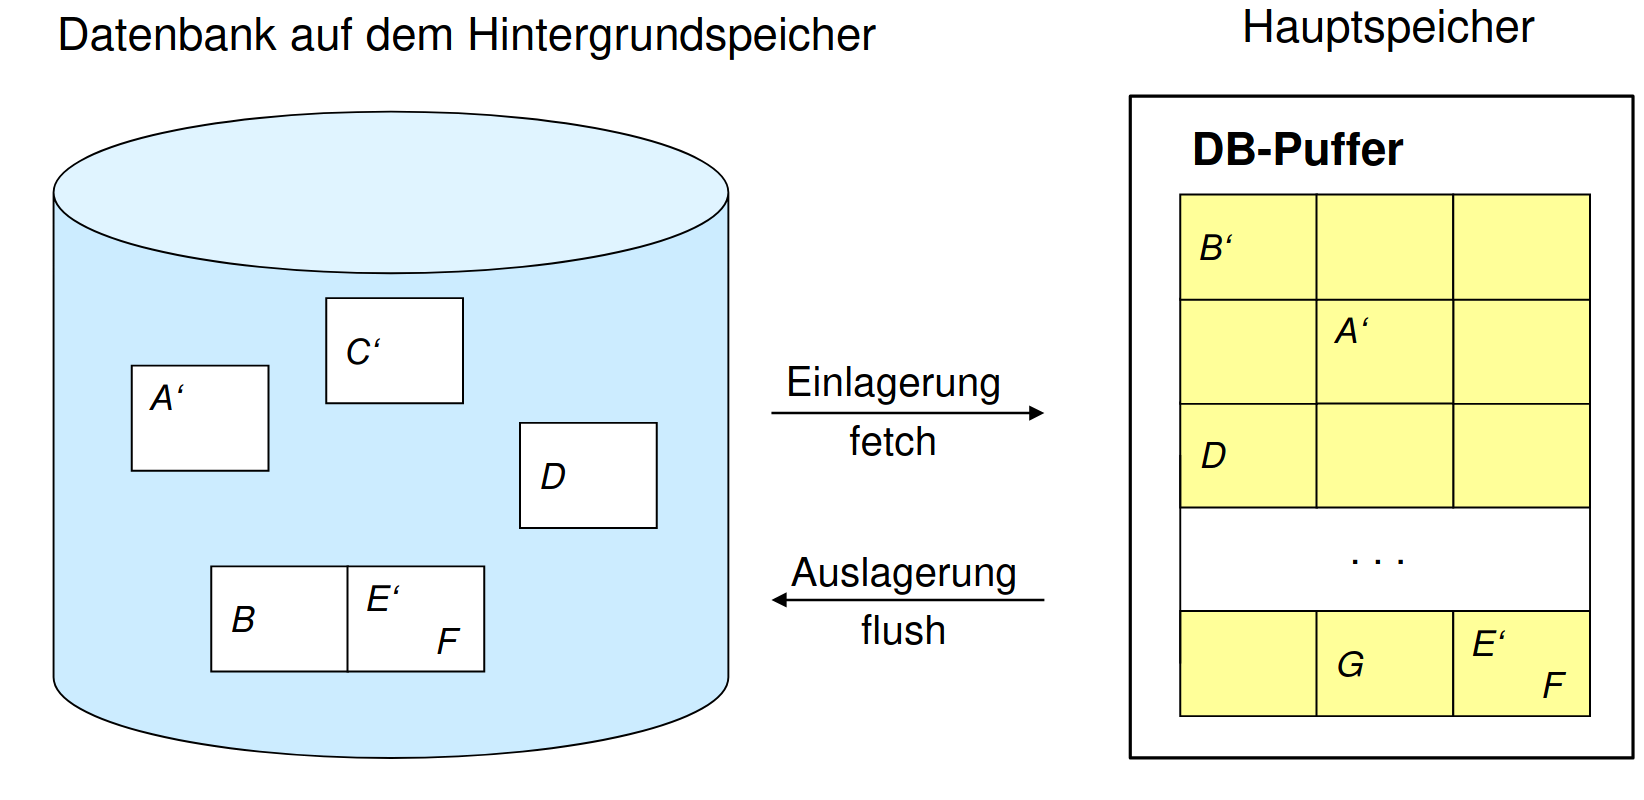
\includegraphics[height=150px]{DB-Puffer.png}

Das DBMS möchte möglichst schnell auf abgefragte Daten zugreifen können. Um dies zu tun, lädt es einige Daten von der langsameren Festplatte in den schnelleren Hauptspecher. Dies macht natürlich besonders viel Sinn, wenn die dort liegenden Daten häufig abgefragt werden. Folglich ist im DBMS komplexe Logik vorhanden, die versucht möglichst effiziente \textbf{Caching-Strategien} umzusetzen. \\

Das DBMS führt auch Statistiken über den Zugriff. Das bedeutet, dass konkret auch die Anzahl der Zugriffe und die Anzahl der Cache-Hits getrackt wird, sodass die Effizienz des Caching Verfahrens analysiert werden kann. Die Statistiken sind in DBMS-spezifischen internen Tabellen abgelegt, die auch abgefragt werden können.

\subsection{Zugriffsarten}

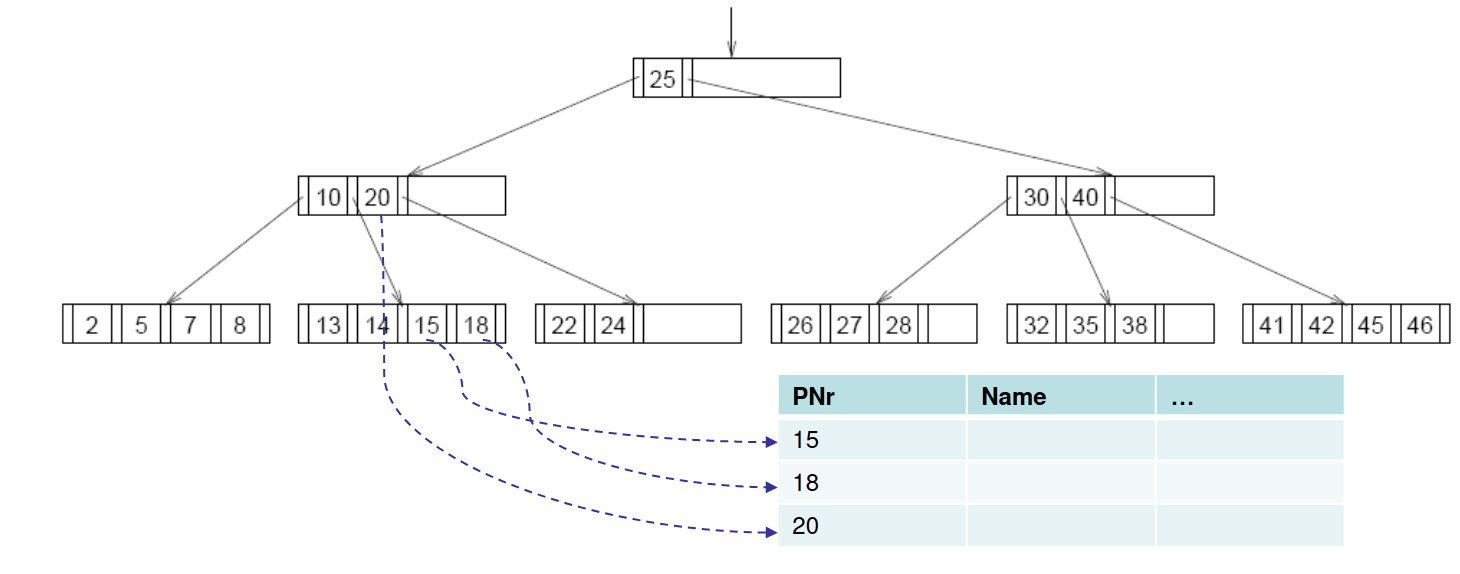
\includegraphics[height=150px]{B-Tree.png}

\textbf{B-Tree}, balanced tree, ist eine Datenstruktur, die zur effizienten Suche benutzt werden kann. In jedem Knoten werden Elemente sortiert abgelegt. Kind-Knoten werden so gelinkt, dass sie jeweils nur Elemente enthalten, die in der Sortierung zwischen zwei Elementen des Eltern-Knoten liegen. Jeder Knoten hat eine maximale Anzahl an Elementen, die er enthalten kann, bevor Elemente in ein neues Kind ausgelagert werden. Innerhalb der Knoten kann eine lineare Suche durchgeführt werden, die aufgrund der niedrigen Anzahl der Elemente trotzdem performant ist. Durch die verschiedenen Stufen des Baumes kann der Bereich, in welchem sich das gesuchte Element befindet, schnell eingegrenzt werden, sodass nur ein Bruchteil des gesamten Baumes mit linearer Suche durchlaufen werden muss. \\
Der B-Tree eignet sich offensichtlich auch gut für Bereichsanfragen, also Anfragen bei denen alle Elemente in einem bestimmten Bereich, der sich auf das Sortierkriterium bezieht, abgefragt werden.

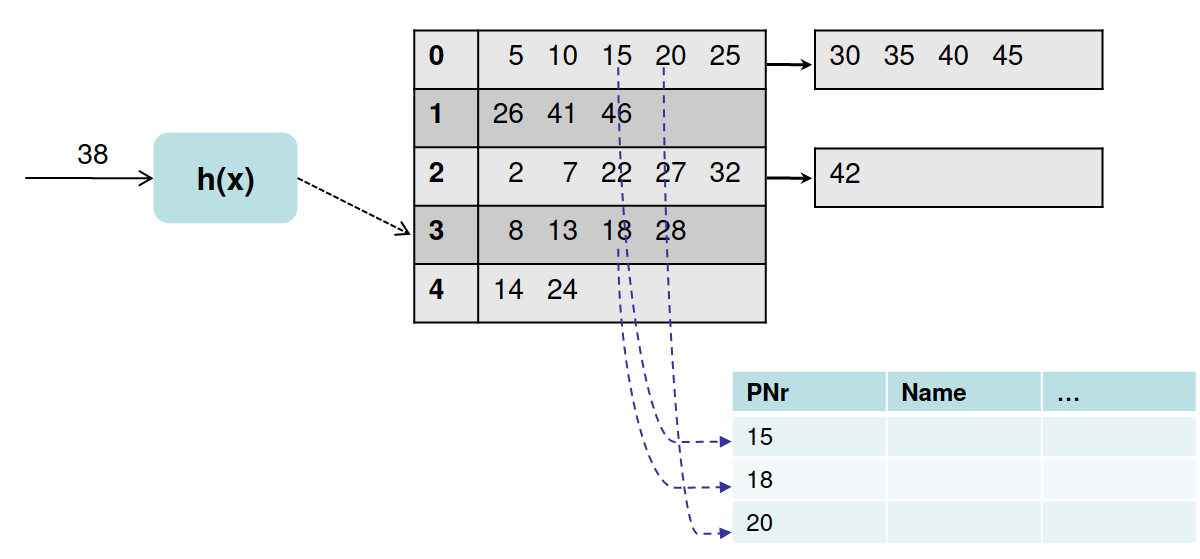
\includegraphics[height=150px]{Hash-Function.png}

\textbf{Hash-Funktionen} sind Funktionen, die eine gegebenenfalls unendlich große Menge von Eingabeelementen auf einen endlich großen Wertebereich abbilden. Die Hash-Funktion soll sehr effizient berechenbar sein, z.B. modulo. Wir können also für ein gegebenes Element den Hash-Wert berechnen. Wenn wir die Hash-Werte und die Ihnen zugeordneten vorhandenen Elemente nach dem Hash-Wert sortiert abspeichern, können wir zu einem Hash-Wert schnell alle zugehörigen Elemente finden. Wenn unsere Hash-Funktion die Elemente möglichst gleichmäßig auf die verschiedenen Werte abbildet, ist gewährleistet, dass die Anzahl der Elemente mit dem selben Hash-Wert sehr gering ist. Deshalb können wir effizient die lineare Suche anwenden, um unser gesuchtes Element in den Elementen mit dem selben Hash-Wert zu suchen. \\
Hash-Funktionen sind sehr performant für das Einfügen und Abrufen einzelner Elemente, da nur einmal die Hash-Funktion angewendet werden muss (im Gegensatz zum B-Tree, bei dem man mehrere Stufen durchlaufen muss). Allerdings sind sie für Bereichsabfragen schlecht geeignet, da die Hash-Werte von Elementen in keinem Zusammenhang zu ihrem Bereich (innerhalb einer Sortierung) stehen und somit der Hash-Wert für jedes einzelne Element berechnet werden muss.

\subsection{Optimizer-Strategien}

Der Optimizer ist die Komponente des DBMS, die bestimmt, auf welche Weise ein Query ausgeführt werden soll. Dazu bestimmt er zunächst alle sinnvollen Ausführungspläne für die Query. Diese Ausführungspläne zeichnen sich durch die Art und Reihenfolge der Operationen aus, sowie durch die dafür verwendeten Technologien (z.B. B-Tree vs. Hash). Dann entscheidet er sich für den aus seiner Sicht besten Ausführungsplan. Die Wahl, die der Optimizer trifft, hängt im Wesentlichen auch von den ihm zur Verfügung stehenden Mittel ab, also z.B. den Indexen. Der Optimizer führt auch Statistiken über die Distribution der Inhalte in den Tabellen, sodass er aufgrund dieser Information Rückschlüsse über die Effizienz von bestimmten Verfahren ziehen kann. Z.B. kann es sein, dass die gleiche Query mit den gleichen Indexen bei verschiedenen Datenbeständen unterschiedlich ausgeführt wird. Konkret ist nämlich das Benutzen eines Hash-Indexes nur dann performanter als eine lineare Suche, wenn auch so viele Daten vorliegen, dass die Daten auf verschiedene DB-Seiten verteilt werden. So wird der Optimizer wahrscheinlich beim Abfragen von Daten aus einer Tabelle mit 10 Einträgen keinen Index verwenden, auch wenn er vorhanden ist. Hingegen wird er mit Sicherheit einen Index verwenden, wenn es 5000 Einträge in der Tabelle gibt. \\

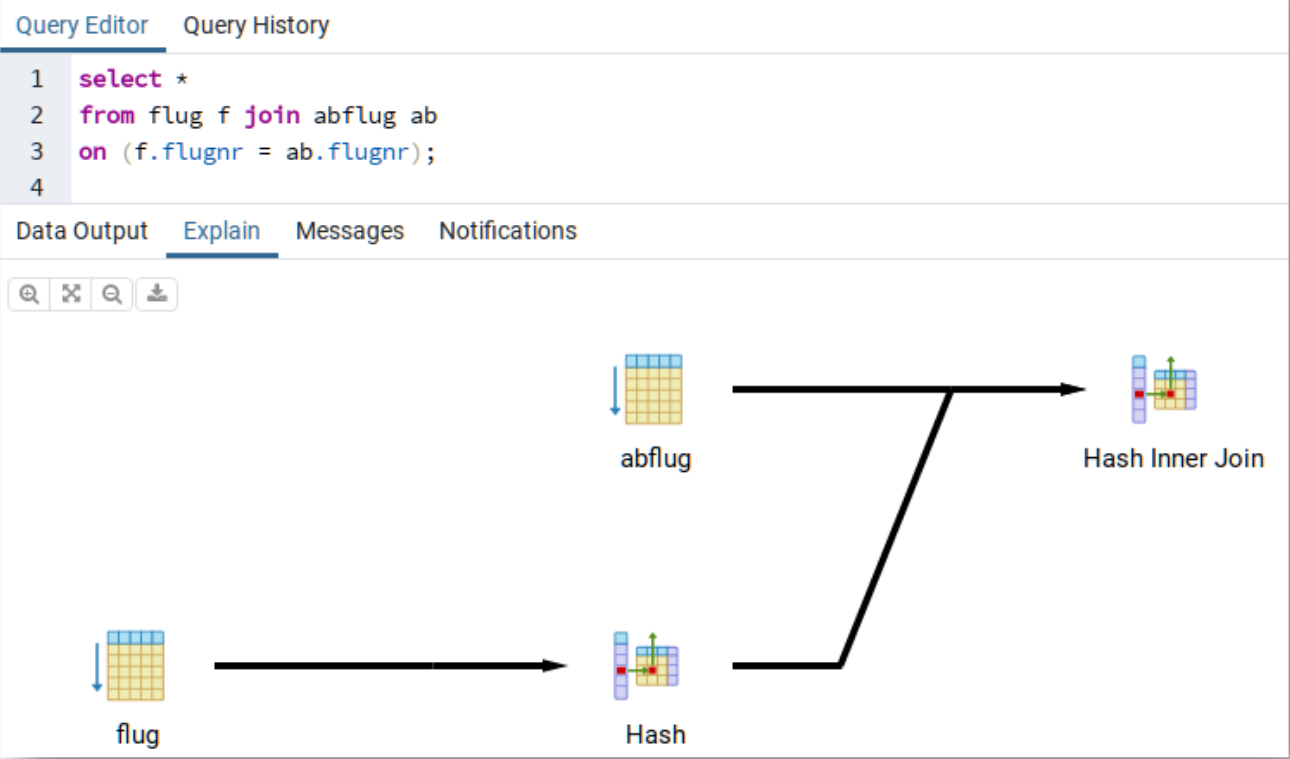
\includegraphics[height=150px]{Explain-Select.png}

Man kann das DBMS auch anweisen, anzuzeigen welchen Ausführungsplan es für eine bestimmte Query benutzen würde. Die Syntax ist hierfür:
\begin{lstlisting}[language=SQL]
    EXPLAIN SELECT ...
\end{lstlisting}

Viele DB-Clients können den Ausführungsplan auch grafisch anzeigen. Im oberen Bild sehen wir ein Beispiel davon für pgAdmin.